%------------------------------------------------------------------------------
% Template file for the submission of papers to IUCr journals in LaTeX2e
% using the iucr document class
% Copyright 1999-2013 International Union of Crystallography
% Version 1.6 (28 March 2013)
%------------------------------------------------------------------------------

\documentclass[preprint,dvipsnames]{iucr}              % DO NOT DELETE THIS LINE



\usepackage{amsmath}
\usepackage{gensymb} % this is for  (\degree) symbol
\usepackage{dcolumn} % for column d in table
\usepackage[normalem]{ulem}
\usepackage{adjustbox}
\usepackage{bm} % for column d in table

%%plot setup%%
\usepackage{pgfplots}
 \pgfplotsset{width=0.7\textwidth,height=0.3\textheight,compat=newest}
 \usetikzlibrary{matrix}
  \usepackage{graphicx}
  \usepackage[referable]{threeparttablex}

\usepackage{epstopdf}
%\usepackage{caption}

%\usepackage[dvipsnames]{xcolor}

% Chemistry
\usepackage[version=3]{mhchem}% <---
\usepackage{textcomp}



\newcolumntype{d}{D{.}{.}{-1}}



% Useful Symbols ...
\newcommand{\B}[1]{\bm{#1}}
\newcommand{\s}[1]{{\textrm{#1}}}
\newcommand{\dg}{$^\circ$}
\newcommand{\A}{\AA}
\newcommand{\pd}[2]{\displaystyle\frac{\partial #1}{\partial #2}}
\newcommand{\pdd}[3]{\displaystyle\frac{\partial^2 #1}{\partial #2 \partial #3}}
\newcommand{\pddd}[4]{\displaystyle\frac{\partial^3 #1}{\partial #2 \partial #3 \partial #4}}
\newcommand{\bra}[1]{\langle#1|}                   % <1|
\newcommand{\ket}[1]{|#1\rangle}                   % |1>
\newcommand{\braket}[2]{\langle#1|#2\rangle}       % <1|2>
\newcommand{\ketbra}[2]{|#1\rangle\langle#2|}      % |1><2|
\newcommand{\braopket}[3]{\langle#1|#2|#3\rangle}  % <1|2|3>
\newcommand{\me}[3]{\left(#2\right)_{#1#3}}        % 2_{13}
\newcommand{\expectation}[1]{\left\langle #1 \right\rangle}   % <1>
\renewcommand{\bar}[1]{\overline{#1}}               % math space
\newcommand{\minus}{\operatorname{-}}
\newcommand{\plus}{\operatorname{+}}
\newcommand{\ci}{\textbf{\textcolor{red}{citation}}{~}}
\newcommand{\ulf}[1]{\textcolor{blue}{#1}}
\newcommand{\justin}[1]{\textcolor{green}{#1}}
\newcommand{\esko}[1]{\textcolor{SkyBlue}{#1}}
\newcommand{\changed}[1]{\textcolor{ForestGreen}{#1}}







     %-------------------------------------------------------------------------
     % Information about journal to which submitted
     %-------------------------------------------------------------------------
     \journalcode{M}              % Indicate the journal to which submitted
                                  %   A - Acta Crystallographica Section A
                                  %   B - Acta Crystallographica Section B
                                  %   C - Acta Crystallographica Section C
                                  %   D - Acta Crystallographica Section D
                                  %   E - Acta Crystallographica Section E
                                  %   F - Acta Crystallographica Section F
                                  %   J - Journal of Applied Crystallography
                                  %   M - IUCrJ
                                  %   S - Journal of Synchrotron Radiation
%%%%%%%%%%%%%%%%
\begin{document}                  % DO NOT DELETE THIS LINE
%%%%%%%%%%%%%%%%




     % The title of the paper. Use \shorttitle to indicate an abbreviated title
     % for use in running heads (you will need to uncomment it).





\title{fragHAR: towards {\em ab initio} quantum crystallographic 
X-ray structure refinement for polypeptides and proteins}

%\shorttitle{Short Title}

     % Authors' names and addresses. Use \cauthor for the main (contact) author.
     % Use \author for all other authors. Use \aff for authors' affiliations.
     % Use lower-case letters in square brackets to link authors to their
     % affiliations; if there is only one affiliation address, remove the [a].


  

\author[a]{Justin}{Bergmann}
\author[b]{Max}{Davidson}
\author[c]{Esko}{Oksanen}
\cauthor[a]{Ulf}{Ryde}{ulf.ryde@teokem.lu.se}{address if different from \aff}
\cauthor[b]{Dylan}{Jayatilaka}{dylan.jayatilaka@uwa.edu.au}{address if different from \aff}

\aff[a]{
Department of Theoretical Chemistry,
Chemical Center,
Lund University,
P.O. Box 124, 
S-22100 Lund, Sweden}

\aff[b]{
School of Molecular Sciences M310,
University of Western Australia,
35 Stirling Highway,
Crawley 6009, Australia}
\aff[c]{
Instruments Division,
European Spallation Source ESS ERIC,
P. O. Box 176, 
SE-221 00 Lund, Sweden}


     % Use \shortauthor to indicate an abbreviated author list for use in
     % running heads (you will need to uncomment it).

%\shortauthor{Soape, Author and Doe}

     % Use \vita if required to give biographical details (for authors of
     % invited review papers only). Uncomment it.

%\vita{Author's biography}

     % Keywords (required for Journal of Synchrotron Radiation only)
     % Use the \keyword macro for each word or phrase, e.g. 
     % \keyword{X-ray diffraction}\keyword{muscle}

%\keyword{keyword}

     % PDB and NDB reference codes for structures referenced in the article and
     % deposited with the Protein Data Bank and Nucleic Acids Database (Acta
     % Crystallographica Section D). Repeat for each separate structure e.g
     % \PDBref[dethiobiotin synthetase]{1byi} \NDBref[d(G$_4$CGC$_4$)]{ad0002}

%\PDBref[optional name]{refcode}
%\NDBref[optional name]{refcode}

\maketitle                        % DO NOT DELETE THIS LINE



% \begin{synopsis}
% Supply a synopsis of the paper for inclusion in the Table of Contents.
% \end{synopsis}


\newpage
\begin{abstract}
We describe the first {\em ab initio} aspherical 
\changed{structure refinement against experimental
X-ray structure factors} for polypeptides and proteins, 
using a fragmentation approach 
to break up the protein into residues and solvent, and thereby speed up 
quantum-crystallographic Hirshfeld atom refinement (HAR) calculations.
We find that the geometric and atomic displacement parameters 
from the new fragHAR method are essentially unchanged 
from a HAR refinement on the complete unfragmented system
when tested on di-, tri- and hexapeptides. The largest
changes are for parameters describing hydrogen atoms involved
in hydrogen-bond interactions, but we show that these discrepancies 
can be removed by including the interacting fragments as
a single larger fragment in the fragmentation scheme.
Significant speedups are observed for the larger systems.
With this approach we are able to perform a highly parallelized 
HAR in reasonable times for large systems. 
The method is implemented in the TONTO software.

\end{abstract}





\newpage

%\input{introduction/introduction.tex}
%\input{theorey/theorey.tex}
%\input{results/refinement_details.tex} %
%\input{Conclusions/Conclusions.tex}




\section{Introduction}

In order to understand the function of proteins and to control or modify enzyme reactions, {\em e.g.} 
by drugs or by mutations, it 
is important to know the detailed atomic structure.  
The most common way to obtain this kind of
information is through X-ray diffraction of protein crystals.
Unfortunately, hydrogen atoms are typically not discerned in protein crystal structures because they have only one electron and therefore scatter X-rays  weakly. 
This is problematic because the hydrogen atoms determine the charge and protonation state of many molecules and residues, and they determine the direction of hydrogen bonds, which are crucial both for the structure of proteins and for the catalytic mechanisms of enzymes.
Therefore, neutron single-crystal diffraction experiments are used as a gold standard to obtain hydrogen positions. Unfortunately, they are more expensive and time-consuming than X-ray crystallographic experiments and sometimes even impossible because large crystals are needed.

At an ultra-high resolution ($<$1 \AA), well-ordered hydrogen atoms start to be visible in crystal structures.
However, protein crystals scarcely scatter to such a resolution -- 
only 671 (0.4\%) data sets in the PDB are in this resolution range.
Moreover, such structures typically give \ce{X-H} bond lengths that are systematically too short (by $\sim$0.12 \AA). The reason for this is that most protein crystallographic 
refinement software employ the independent atom model (IAM) 
to obtain atom positions and displacement parameters.  
IAM uses a superposition of smeared {\em spherical} atomic densities
to describe the averaged electron 
density in the periodic crystal~\cite{coppens1997x}.
However, the electron density of a hydrogen atom is not spherical and it is not centred on the nucleus. Instead, the maximum of the electron density in a \ce{X-H} bond is shifted 
from the nuclei of the hydrogen atom into the bond.   
The atomic displacement parameters (ADPs) of the hydrogen atoms
are even more difficult to obtain correctly in X-ray crystal structures. In fact, the positions of  
non-hydrogen atoms with lone pairs may also be shifted slightly, another example of a non-spherical electron density. 





% Aspherical for hydrogen refinement & QCr
Fortunately, there are methods to obtain accurate hydrogen-atom 
positions and ADPs from X-ray diffraction data, based on an aspherical electron-density description of the atoms, but so far available only for small molecules
with a resolution of $<$0.85 \AA.
\citeasnoun{destro1995bond} were the first to demonstrate 
that this is possible using the Hansen--Coppens multipole model 
and several others have used the same approach
\cite{zhurov2011importance,zhurov2013charge}. 
\citeasnoun{dittrich2005invariom} showed that it is possible 
to obtain \ce{X-H} bond lengths in agreement with those obtained by neutron structures using 
a database of aspherical atomic form factors fitted to structure factors
obtained from a quantum-chemical (QM) calculations.
\changed{Very recently, \citeasnoun{Malaspina2019} have reported a
quantum-mechanical database for chemical fragments that can be used to build 
a whole protein, which also recovers
excellent X-H bond lengths}.



Hirshfeld atom refinement (HAR) is a method that
allows the determination of hydrogen-atom positions 
from standard-resolution small-molecule X-ray crystallography
\cite{jayatilaka2008x,capelli2014hirshfeld}.
In HAR,  a wavefunction for the molecule in the crystal geometry 
is calculated. From this wavefunction, an electron density (ED)
is obtained,  which is then partitioned into aspherical atomic pieces 
using Hirshfeld's stockholder  partitioning scheme. The aspherical 
atomic structure factors, {\em i.e}. the Fourier transform of the Hirshfeld atomic ED, 
are then calculated and used in a least-squares refinement  
against the \changed{experimental X-ray structure factors}. 
HAR has the advantage that  it does not require any 
aspherical form factors stored in databases or tables. 
Neither are the aspherical atomic form factors approximated using multipoles. 
Instead, they are calculated by QM methods when required.
With HAR, hydrogen-atom  positions can be obtained in quantitative 
agreement with neutron diffraction results even at 0.8 {\AA} 
resolution \cite{woinska2016hydrogen}.
\changed{It should be emphasised that non-hydrogen atom positions 
obtained from HAR are more precise than can be obtained from quantum 
chemical energy optimisations---even with high level methods}.


% Practical problems
Unfortunately, there is no free lunch: HAR is many orders of magnitude 
slower than IAM and database  methods. In particular, the time consumption 
increases sharply with the size of the studied system, because calculating 
a QM wavefunction is very time consuming for large molecules. This makes HAR 
currently unfeasible for large systems like polypeptides and proteins. 

Of course, the
problem of performing QM calculations on large systems 
has occupied quantum chemists for a long time and
many techniques have been developed, including methods 
that are linear-scaling in the number of atoms.



A well-established approach for modelling proteins is the QM/MM method, 
which describes a region of interest {\em e.g.} the active site with a 
QM method and the remainder 
with a molecular 
mechanics (MM) model~\cite{warshel1976theoretical,singh1986combined,
Thiel:09,Ryde:qmmmrev}.  QM/MM methods can be used 
for the refinement of low- and medium-resolution protein structures, when combined with the joint X-ray/MM refinement 
method of \citeasnoun{brunger1987crystallographic}. The result is the 
quantum-refinement method of \citeasnoun{ryde2002quantum}. 
Merz and coworkers have suggested a similar method, in which the complete protein is described by
semiempirical quantum mechanical calculations~\cite{Merz:05}. Importantly, this
method has been integrated into the widely used Phenix protein structure 
refinement program \cite{borbulevych2014accurate}.  
\changed{An alternative approach,  Q$\vert$R, has also been suggested, 
in which the full protein is treated by density-functional 
theory~\cite{zheng2017q}. Still, all these methods 
make use of spherical atomic form factors.}

Another way to speed up the QM calculations is to fragment the full 
system into smaller subsystems, for which the wavefunction is calculated, 
and then ``piece'' the results together. This approach, which is obviously 
linear scaling, makes QM calculations feasible for 
proteins~\cite{stoll1992correlation,doll1997quantum,zhang2003molecular,soderhjelm2008accurate,%
yang1991direct,lee1996linear,yang1995density,kohn1996density,%
dixon1996semiempirical,gogonea2000quantum,stewart1996application,%
daniels1997semiempirical,daniels1999best,scuseria1999linear}.
These methods have been reviewed by \citeasnoun{collins2015energy},
\changed{and a general program to implement it by scripting other
{\em ab initio} packages has been presented by \citeasnoun{Kobayashi2019}}.

All these methods focus on obtaining the {\em energy}, whereas
the ED, if it is produced at all, is just a byproduct. 
\citeasnoun{walker1994ab} have reported 
a Mulliken-like method to produce EDs for proteins
from fragments, but it has not been used for X-ray structure 
refinement. \citeasnoun{massa1995quantum} has proposed the
kernel density method to obtain the ED of large systems 
and has applied it to a cyclic hexapeptide whose structure 
was taken from X-ray measurements, 
but no  X-ray structure refinement was attempted.
Very recently, \citeasnoun{northey2019ab} developed a 
fragmentation approach for ED calculated by the ab initio X-ray 
diffraction method, fitted to X-ray free-electron laser data,
and \changed{\citeasnoun{Malaspina2019} et al.
have derived a database of extremely localised molecular
orbitals for chemical fragments which can be used
to build a protein and permit large HAR calculations, a method
called HAR-ELMO}.


In this paper, we develop a fragmentation approach to
speed up the QM protein structure-factor calculations 
required for HAR with single-crystal data. 
It is based on the molecular fractionation
with conjugate caps (MFCC) approach of \citeasnoun{zhang2003molecular}.
Our method, which we call fragHAR,
is described in the next section, and is tested on three oligopeptides 
systems for which high-quality X-ray diffraction data are 
available: a dipeptide, a tripeptide, and a hexapeptide. 
The results are compared against full HAR calculations;
\changed{the accuracy of HAR relative to neutron diffraction 
measurements has already been
established~\cite{capelli2014hirshfeld,fugel2018probing}}.


\section{Theory and Methods}

\subsection{Hirshfeld atom refinement }

The HAR calculations were performed as described in the literature \cite{jayatilaka2008x,%
capelli2014hirshfeld,woinska2014hirshfeld}.
The atomic form factors were calculated numerically using Becke integration grids \cite{becke1988multicenter}.
The least-squares procedure is performed using
standard methods, refining against the structure-factor magnitudes,
and no attempt were made to parallellize this part of the code, because it does not limit the calculations for the small systems considered here. 
All calculations were performed with a development version of the TONTO software~\cite{tonto}.



\subsection{The fragHAR fragmentation scheme}
\label{sec_frag}

\citeasnoun{zhang2003molecular} introduced a method to achieve 
a linear scaling for the calculation of the QM energy of proteins,
called molecular fractionation with conjugate caps.
This method breaks a protein into residues by cutting the 
peptide bonds and replacing the \ce{RNH-} group with \ce{CH3NH-},
and the \ce{R^{'}C=O} group with \ce{CH3C=O}. Larger fragments 
may also be used \cite{grimme:12}, but as we show below, 
this procedure works well for X-ray structure refinement.

Truncating hydrogen atoms are placed in the direction 
of the actual atoms at standard distances \cite{allen2010bond}. 
The fragmentation scheme is illustrated schematically in Figure \ref{fig_fragmentation}
for a dipeptide. 
Solvent molecules are treated as separate fragments. 
 
In our implementation, bonded atoms are defined according to 
the Cambridge Crystallographic Database criterion,
\begin{align}
d_\s{AB} < r_\s{A} + r_\s{B} + 0.4
\label{eq_bond}
\end{align}
where $r_\s{A}$ and $r_\s{B}$ are the covalent radii of atoms A and B,
respectively, and $d_\s{AB}$ is the distance between them (all in \AA). Using this 
criterion, hydrogen bonds are not taken into account, but such  
connections are easy to introduce by instead using van der Waals radii in 
equation \ref{eq_bond}. 
The assumption that only next-nearest neighbour 
non-hydrogen atoms are sufficient to provide a good model of the ED
central fragment was established already 
by \citeasnoun{dittrich2002reproducability}.
This scheme is easily generalised, if required. 

In our fragHAR approach, structure factors are calculated for the central (non-overlapping) part of each fragment ({\em i.e.} for each residue separately), using the wavefunction for each capped fragment. 
These structure factors are then directly employed in the standard HAR procedure, without any modification.
Thus, there is no need to calculate structure factors for any conjugate capping groups.

%\begin{figure}
%   \begin{tiny}
%     \chemfig{[:30]\color{ForestGreen}{^+H_3N}-[,,,,,ForestGreen]([::60]-[,,,,,ForestGreen]\color{ForestGreen}{R_1})-[::-60,,,,,ForestGreen](=[::-60,,,,,ForestGreen]\color{ForestGreen}{O})-[::60]\color{CornflowerBlue}{N}([::60,,,,,CornflowerBlue]-\color{CornflowerBlue}{H})-[::-60,,,,,CornflowerBlue](-[::-60,,,,,CornflowerBlue]\color{CornflowerBlue}{R_2})-[::60,,,,,CornflowerBlue]\color{CornflowerBlue}{COO^{-}} }
%     $\longrightarrow$ 
%     %
%     %
%     \chemfig{[:30]\color{ForestGreen}{^+H_3N}-[,,,,,ForestGreen]([::60]-[,,,,,ForestGreen]\color{ForestGreen}{R_1})-[::-60,,,,,ForestGreen](=[::-60,,,,,ForestGreen]\color{ForestGreen}{O})-[::60]\color{BurntOrange}{N}([::60,,,,,BurntOrange]-\color{BurntOrange}{H})-[::-60,,,,,BurntOrange]\color{BurntOrange}{CH_3} } 
%     +
%     %
%     %
%     \raisebox{\baselineskip}{
%       \chemfig{\color{RubineRed}{H_3C}-[:-30,,,,,RubineRed](=[::-60,,,,,RubineRed]\color{RubineRed}{O})-[::60]\color{CornflowerBlue}{N}([::60,,,,,CornflowerBlue]-\color{CornflowerBlue}{H})-[::-60,,,,,CornflowerBlue](-[::-60,,,,,CornflowerBlue]\color{CornflowerBlue}{R_2})-[::60,,,,,CornflowerBlue]\color{CornflowerBlue}{COO^{-}} }
%       }
%   \end{tiny}
%         
%   \caption{Example illustrating the MFCC procedure for cutting a dipeptide
%   (left hand side) across the peptide bond (shown in black) producing 
%   two fragment molecules (right hand side) which are capped with \ce{-COCH3}
%   (\textcolor{RubineRed}{red}) and \ce{-NHCH3} (\textcolor{BurntOrange}{orange}) 
%   groups, comprised of the neighbour and next-neighbour non-hydrogen atoms. }
%   \label{fig_fragmentation}
%   
%\end{figure}

\begin{figure}
 \centering
 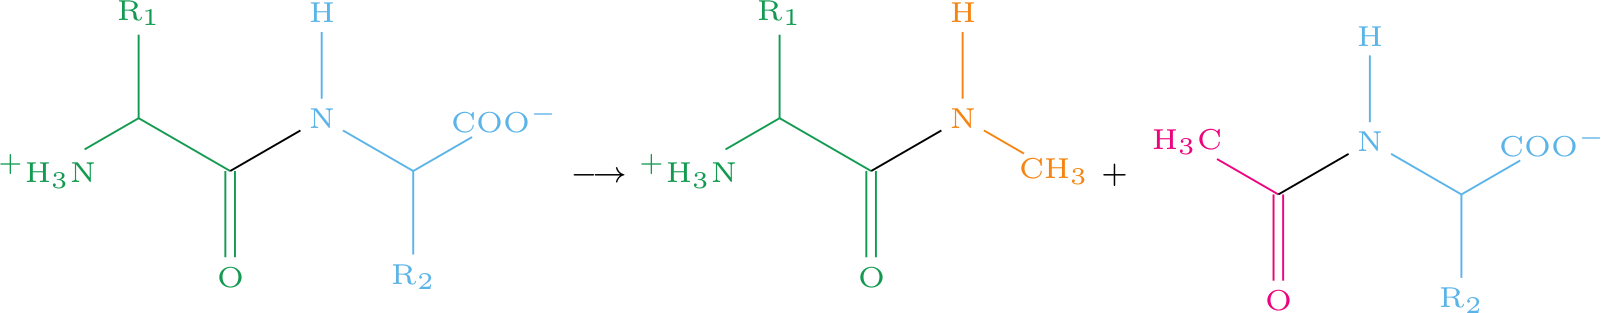
\includegraphics[width=0.8\linewidth]{MFCC.png}
 
 \caption{The Molecular Fractionation with Conjugate Caps (MFCC) 
 procedure for cutting a dipeptide (left hand side) across the 
 peptide bond (shown in black) producing two fragment molecules 
 (right hand side) which are then ``capped'' with \ce{-CH3C=O}
 (\textcolor{RubineRed}{red}) and \ce{-NHCH3} (\textcolor{BurntOrange}{orange}) 
 groups, comprised of the neighbour and next-neighbour non-hydrogen atoms. }
 \label{fig_fragmentation}
 
\end{figure}



An important difference concerning energy fragmentation methods 
versus electron-density fragmentation methods is that for X--ray 
structure refinement, only the aspherical atomic structure
factors are required. Therefore, there is no need to subtract the energies
of the capping groups \cite{zhang2003molecular}). 



\subsection{Parallelization and timing}

For large systems, the fragmentation scheme will of course
speed up the aspherical atomic structure-factor calculations
because the %wavefunction 
calculations are performed on smaller
molecules; the time will be no more than $N_\s{frag}$ times the calculation
time for the largest fragment, {\em i.e.} linear scaling in the number
of fragments $N_\s{frag}$. Provided the least-squares
procedure is not a bottleneck, a fixed calculation time
may be achieved if each of these fragment calculations is
performed in parallel on separate processors. 
We have implemented such a parallelization using the MPI
protocol, whereby the QM calculations on each fragment are
distributed to free processors as soon as they become available.

\subsection{Choice of model systems and experimental data}

Three published test systems were used to show that the  
fragmentation is a reasonable approximation to get a good refined structure.
The systems were the dipeptide Gly--Ala (GA) \cite{capelli2014hirshfeld}, 
the tripeptide  Ala--His--Ala (AHA; with 2-Propanol and water as solvent)~\cite{grabowsky2009transferability} and 
the hexapeptide cyclo-(Ala)\textsubscript{4} --(D,L-Pro)\textsubscript{2} 
(\ce{A4P2}; with one water molecule as solvent) \cite{dittrich2002reproducability}. 
The solvent molecules were treated as separate fragments in fragHAR.
As reference, a full HAR calculation with a single wavefunction for the complete structure was used.


\begin{figure}

 \centering
 
 \begin{minipage}[t]{0.26\linewidth}
  \centering
 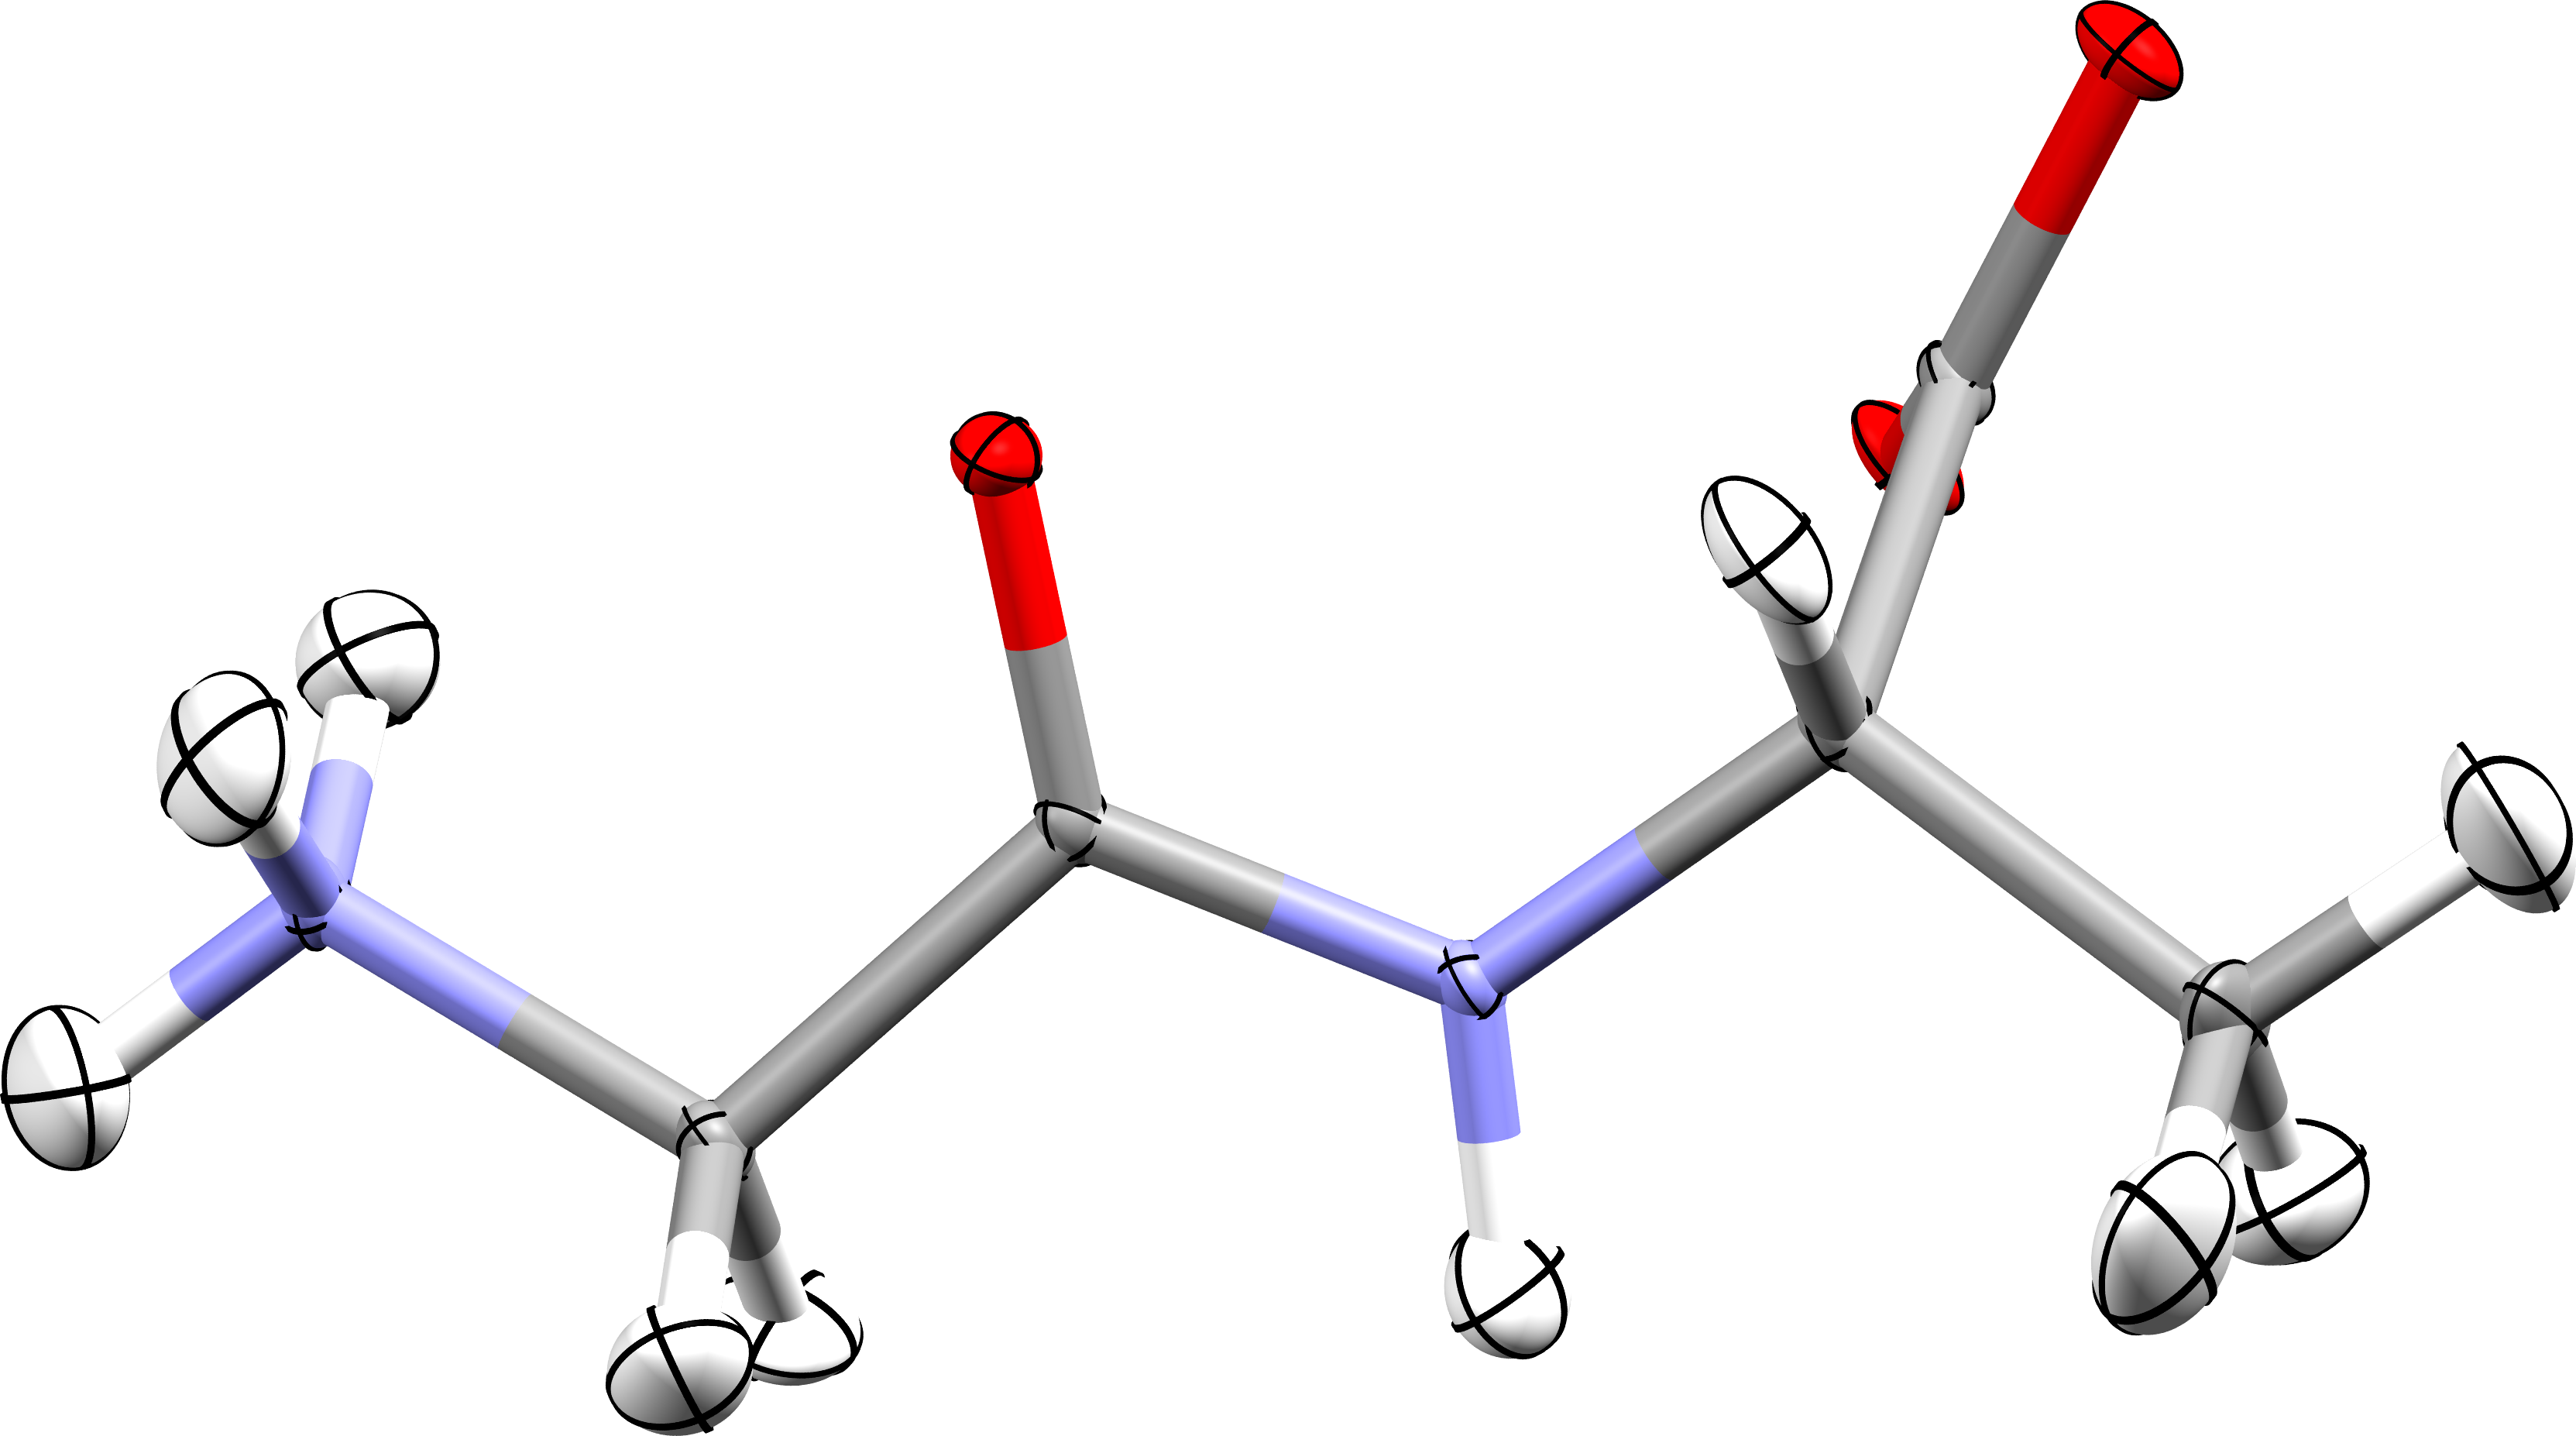
\includegraphics[width=1\linewidth]{glyala.png}
 (a) Gly-Ala (GA)
\end{minipage}%
  \begin{minipage}[t]{0.36\linewidth}
 \centering
 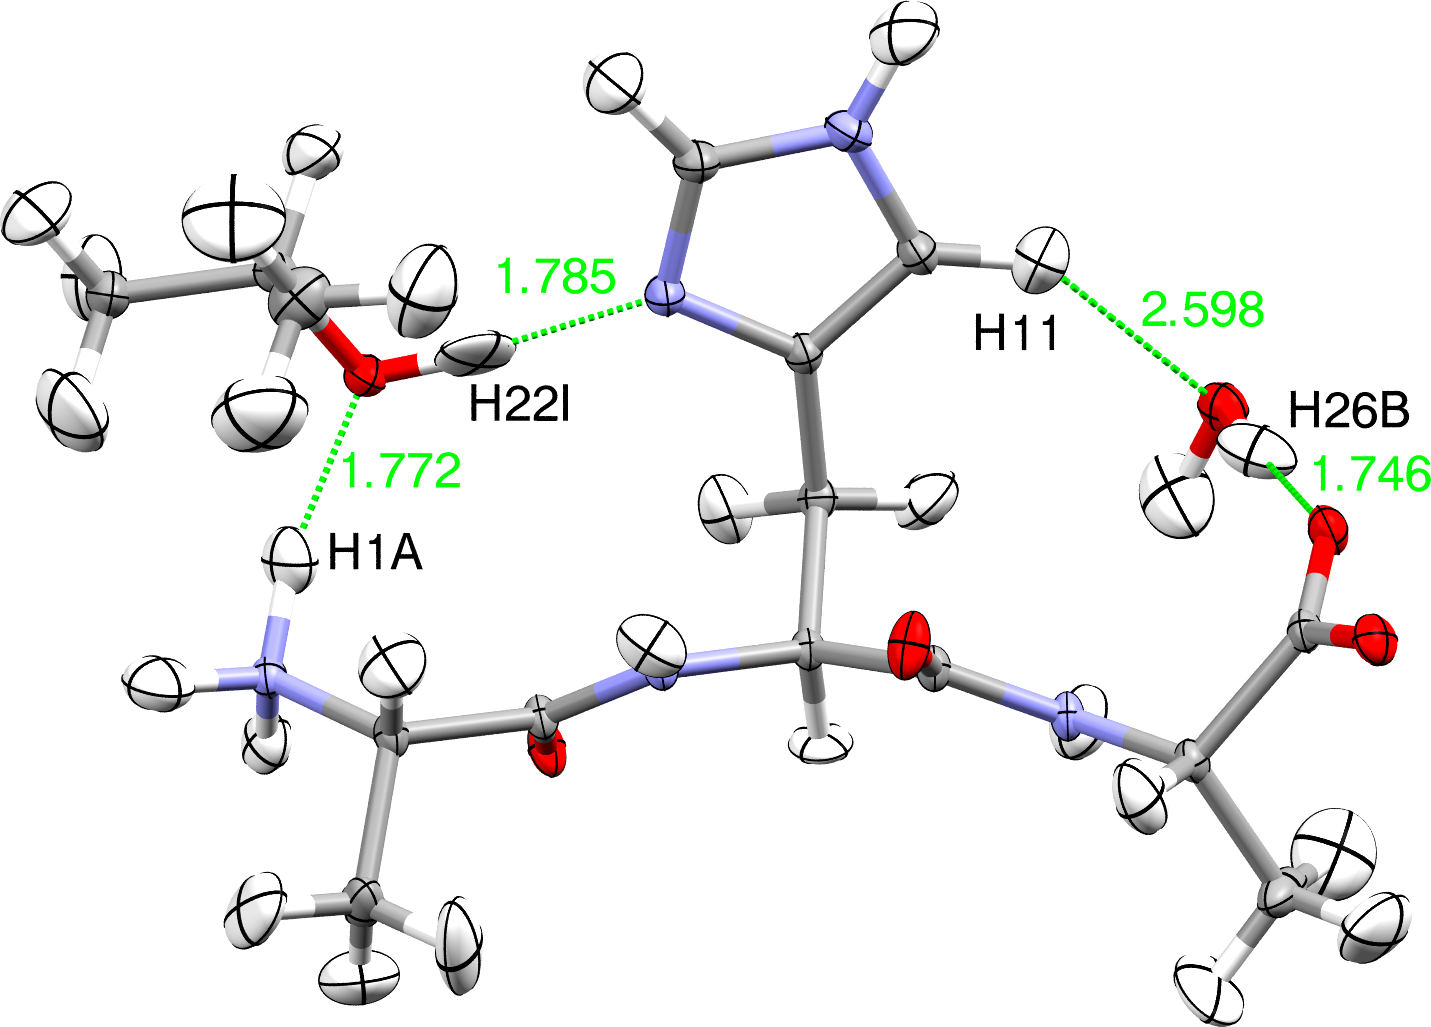
\includegraphics[width=1\linewidth]{AHA.png}
 (b) Ala-His-Ala (AHA)
 \end{minipage}%
  \begin{minipage}[t]{0.36\linewidth}
 \centering
 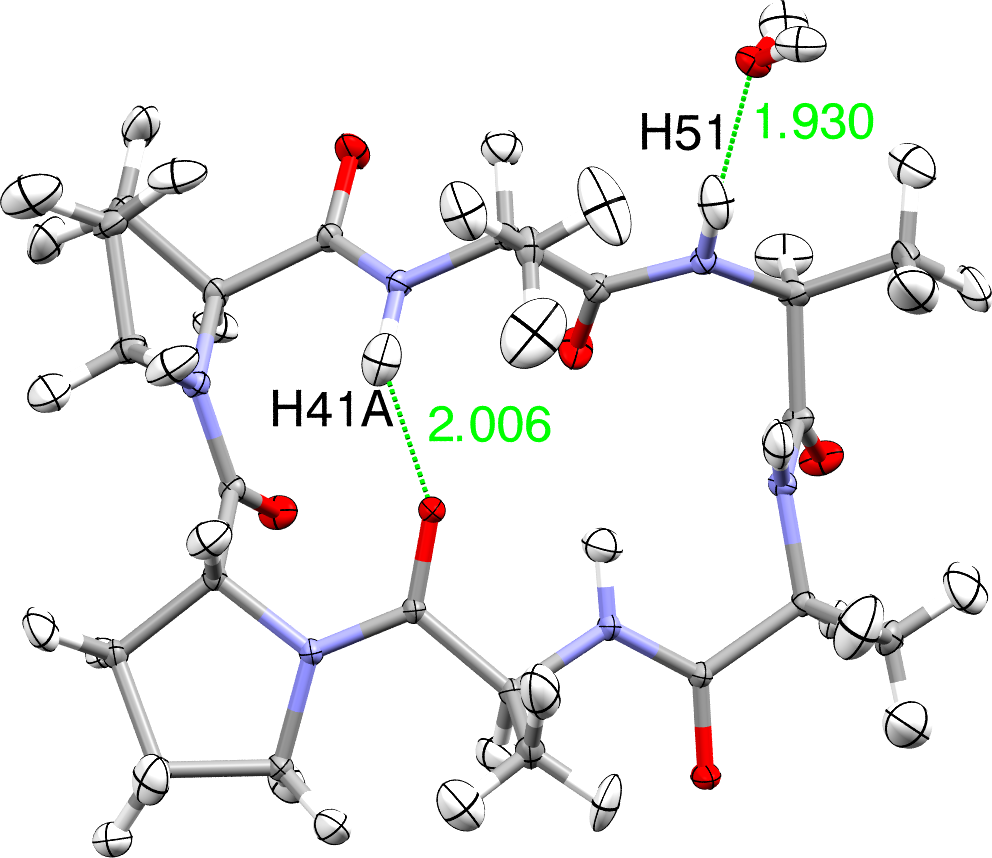
\includegraphics[width=0.9\linewidth]{AAPPAA.png}
 (c) cyclo-(Ala)\textsubscript{4} -(D,L-Pro)\textsubscript{2} (\ce{A4P2})
 \end{minipage}%
 \caption{Crystal structures (100K) of the three peptide model systems 
 with 50\% ADP probability ellispoids. Hydrogen bonds appear in green. }
  \label{fig_model_systems}
\end{figure}




\subsection{Details of wavefunction calculations}

All QM calculations (both for HAR and fragHAR) were performed using 
Hartree--Fock wavefunctions using the cc-pVDZ basis of\cite{dunning1989gaussian}.   
This has previously been found to be a proper level of theory 
\changed{when refining QM wavefunctions to structure factors,}
giving \ce{X-H} bond lengths in agreement with neutron
diffraction results~\cite{capelli2014hirshfeld,fugel2018probing}. 
\changed{Note that the QM calculations are used to obtain 
the aspherical electron density (to calculate  structure factors), 
not to optimise the geometries on a potential energy surface}.



\subsection{Quality statistics}

We use standard crystallographic statistics to compare data sets 
(in our case the fragHAR and HAR refinement)~\cite{schwarzenbach1995statistical}. 
In addition, we use the mean of the ratio of data pairs 
($\langle  r_\s{fragHAR}/r_\s{HAR}\rangle$) and the mean absolute 
difference ($\langle |\Delta r | \rangle = \langle |r_\s{fragHAR}-r_\s{HAR}| \rangle$) 
between the data pairs. To establish statistical agreement
between two parameter sets $\{ A_i \}$  and $\{ B_i \}$ we use 
the weighted root-mean square deviation
~\cite{capelli2014hirshfeld,schwarzenbach1995statistical},
\begin{align}
w\s{RMSD} & = \sqrt{\left< \frac{(A_i - B_i)^2}{(su(A_i)^2 +su(B_i)^2} \right>}
\label{eq_wrmsd}
\end{align}
where $su$ is the standard uncertainty, and values in the range $0 \leq w\s{RMSD} < 1$ 
indicate that the two data sets are in statistical agreement.



\section{Results and Discussion}
\label{sec_results}

\subsection{Comparison of goodness-of-fit parameters}

Table \ref{tbl_cryst} summarizes the crystallographic data and the
refinement results for both the fragHAR and the reference HAR calculations 
for the three tested oligopeptides. It can be seen that there are only 
negligible differences in both the residue density peaks 
(third decimal place) and the $R$ values (second decimal place)
between the two refinements. 




\begin{table}
\caption{Crystallographic refinement details for the fragHAR versus HAR,
including calculation times, 
obtained using Hartree--Fock wavefunctions 
with the cc-pVDZ basis set.\\} 
\label{tbl_cryst}

\begin{tabular*}{\linewidth}{lrrrrrr}
\\
  \hline
   &\multicolumn{2}{c}{GA}&\multicolumn{2}{c}{AHA}&\multicolumn{2}{c}{\ce{A4P2}} \\ 
  \hline
  
  Formula  
  & \multicolumn{2}{c}{\ce{C5 H10 N2 O3}}
  & \multicolumn{2}{c}{\ce{C15 H29 N5 O6}}
  & \multicolumn{2}{c}{\ce{C22 H36 N6 O7}}  \\
   
  System 
  & \multicolumn{2}{c}{Orthorhombic}
  & \multicolumn{2}{c}{Monoclinic}&\multicolumn{2}{c}{Orthorhombic }  \\  
  Group
  & \multicolumn{2}{c}{$P 2_1 2_1 2_1$}
  & \multicolumn{2}{c}{$P 2_1 $}
  & \multicolumn{2}{c}{$P 2_1 2_1 2_1$ }  \\  
   
  $\lambda$/\AA &\multicolumn{2}{c}{0.5259}
  & \multicolumn{2}{c}{0.560}
  & \multicolumn{2}{c}{0.5583 }  \\  
   
$a$/\AA 
  & \multicolumn{2}{c}{7.472(2)}
  & \multicolumn{2}{c}{8.7410(17)}
  & \multicolumn{2}{c}{ 10.1280(10)} \\  
$b$/\AA
  & \multicolumn{2}{c}{9.4907(6)}
  & \multicolumn{2}{c}{9.4200(19)}
  & \multicolumn{2}{c}{12.4860(10)}  \\ 
$c$/\AA 
  & \multicolumn{2}{c}{9.7169(8)}
  & \multicolumn{2}{c}{11.989(2)}
  & \multicolumn{2}{c}{9.5070(10)}  \\  
$\alpha =\gamma$/\textdegree
  & \multicolumn{2}{c}{90}
  & \multicolumn{2}{c}{90}
  & \multicolumn{2}{c}{90 } \\
$\beta$/\textdegree 
  & \multicolumn{2}{c}{90}
  & \multicolumn{2}{c}{95.49(3)}
  & \multicolumn{2}{c}{90 }  \\  
$T$/K&\multicolumn{2}{c}{100(2)}
  & \multicolumn{2}{c}{100(2)}
  & \multicolumn{2}{c}{100(2) }  \\
 $d$/\AA
  & \multicolumn{2}{c}{0.65}
  & \multicolumn{2}{c}{0.43}
  & \multicolumn{2}{c}{0.38 }  \\  
 
$N_\s{meas}$ 
  & \multicolumn{2}{c}{2431}
  & \multicolumn{2}{c}{12261}
  & \multicolumn{2}{c}{22268}  \\  
 $N_\s{atoms}$ 
  & \multicolumn{2}{c}{20}
  & \multicolumn{2}{c}{55}
  & \multicolumn{2}{c}{71}  \\
& \\

                            &fragHAR    &HAR     &fragHAR        &HAR     &fragHAR    &HAR \\
\
   $N_\s{fragments}$ &2&1&5&1&7&1\\
   $\rho_\s{max}$/e\AA$^{-3}$ &0.1487   &0.469      &0.1573     &0.1606     &0.2423     &0.2400   \\
   $\rho_\s{min}$/e\AA$^{-3}$ &-0.1579  &-0.1792    &-0.2000    &-0.1996    &-0.1988    &-0.1967  \\
   $R(F)$/\%                 &1.70      &1.82       &2.41       &2.39       &3.29       &3.29       \\
   $wR(F)$/\%                &1.45      &1.55       &2.10       &2.09       &2.88       &2.89       \\
 \hline
  \end{tabular*}
\end{table}






\subsection{Comparison of bond lengths}

Figure \ref{fig_bond_len_non_H} compares the bond lengths involving non-hydrogen atoms obtained by HAR and fragHAR for the three peptides. It can be seen that the two sets show a perfect agreement. Therefore, we do not present any deeper
statistical analysis (more detailed graphs are provided in the supplementary material). 
Clearly, fragHAR does not represent any significant approximation compared 
to HAR for the non-hydrogen atoms.

Results for the \ce{X-H} bond lengths obtained in the refinements are shown in Table \ref{tbl_bond}. The bond lengths
are divided into three classes, \ce{C-H}, \ce{N-H} and 
\ce{O-H}, in order to make the comparison more detailed.
It can be seen that the \ce{C-H} bond lengths from the two refinements are in statistical agreement ($w\s{RMSD}$ = 0.2--0.8). 
There is a minimal tendency that the fragHAR bond lengths are slightly  shortened ($\langle  r_\s{fragHAR}/r_\s{HAR}\rangle$ = 0.998--0.999), but the deviation from unity is less than the standard uncertainty. 
The \ce{N-H} bond lengths in GA are also in statistical agreement ($w$RMSD = 0.4),
but for the bigger oligopeptides, there is a slight
disagreement in the \ce{N-H} bonds, with $w$RMSDs of 1.2 and 1.0. Likewise, the
\ce{O-H} bond lengths in the tripeptide AHA show a statistical disagreement,
with $w$RMSD = 2.4, whereas the two \ce{O-H} bonds in A$_4$P$_2$ agree between the two methods ($w$RMSD = 0.5).



\noindent
\begin{threeparttable}
\begin{table}

\caption{Comparison of \ce{X-H} bond length obtained with fragHAR and HAR.
Values in brackets represent the sample standard deviations.}
  \label{tbl_bond}
 \begin{tabular*}{\linewidth}{ccclllll}
 \\
 \hline
  Compound
 & Bond  
 & $N_\s{data}$
 & $\langle  r(\ce{X-H})\rangle$ 
 & $\langle  r(\ce{X-H})\rangle$
 & $\langle  r_\s{fragHAR}/r_\s{HAR}\rangle$ 
 & $\langle |\Delta r | \rangle$
 & $w$RMSD \\
 &  & & fragHAR & HAR \\
 \hline
 
 GA  & \ce{ C-H } & 6 & 1.09(2) & 1.09(2) &  0.999(4) & 0.003(4) & 0.40 \\
     & \ce{ N-H } & 4 & 1.03(2) & 1.03(2) &  0.999(3) & 0.002(3) & 0.32 \\

 \\                           
 AHA  & \ce{ C-H } & 20 & 1.11(2) & 1.11(2) &  0.998(9) & 0.007(8) & 0.8 \\
      & \ce{ N-H } & 6 & 1.05(4) & 1.06(4) &  0.99(2) & 0.01(2) & 1.24 \\
      & \ce{ O-H } & 3 & 1.00(4) & 1.02(4) &  0.98(3) & 0.02(3) & 2.4 \\
& \\                          
 \ce{A4P2}  & \ce{ C-H } & 30 & 1.08(3) & 1.08(3) &  0.999(3) & 0.001(2) & 0.18 \\
            & \ce{ N-H } & 4 & 1.00(2) & 1.01(2) &  0.989(8) & 0.01(2) & 0.98 \\
            & \ce{ O-H } & 2 & 0.958(7) & 0.964(7) &  0.994(3) & 0.005(6) & 0.43 \\

 \hline

  \end{tabular*}
  \end{table}
 \end{threeparttable}


To investigate the reason for these differences, we plotted the bond
lengths from fragHAR and HAR in Figure \ref{fig_bond_len_H_bond_type}.
It can be seen that for most bonds, the results of the two methods agree, but there are are a few outliers that are identified by atom labels (explained in Figure \ref{fig_model_systems}).   It can be seen that all the outliers are 
associated with hydrogen atoms involved in intermolecular 
hydrogen bonds between the residues or the solvent molecules. Such interactions are not modelled 
in the fragHAR method with residue fragments.
It is remarkable that 
the X-ray data contains enough information to distinguish these small 
hydrogen bonding effects via their neglect in the fragHAR model.

To see if this shortcoming may be eliminated, we joined the two 
fragments involved in the hydrogen bond of interest
and treated them as a single fragment. 
\changed{Figure \ref{fig_bond_len_H_join_frag} shows that such 
a procedure solves the problem for all X--H bond lengths. 
For example, the N--H41A bond length in \ce{A4P2} 
(H41A makes an intramolecular 
hydrogen bond, as can be seen in Figure \ref{fig_model_systems}) 
improves from 1.000(10)~\AA{} for standard fragHAR, to 1.017(9)~\AA{} 
with the doubled fragment, compared to 1.020(9)~\AA{} for HAR. Therefore,
these small discrepancies can be corrected if
the size of the fragment is increased to include all the
residues that are hydrogen bonded to it. Since the calculations
are performed in parallel the time taken will still be roughly 
equal to time for the largest fragment.}

Finally, we note that both HAR and fragHAR give \ce{X-H} bond 
lengths that are in agreement with those obtained by neutron 
crystallography, in contrast to IAM that gives too short 
\ce{X-H} bond lengths. This illustrates that X-ray data with 
a resolution of less than 0.8 {\AA} can provide as accurate 
hydrogen positions as neutron crystallography~\cite{jayatilaka2008x,woinska2014hirshfeld,%
capelli2014hirshfeld,fugel2018probing}. 




		
\begin{figure}
 \centering
 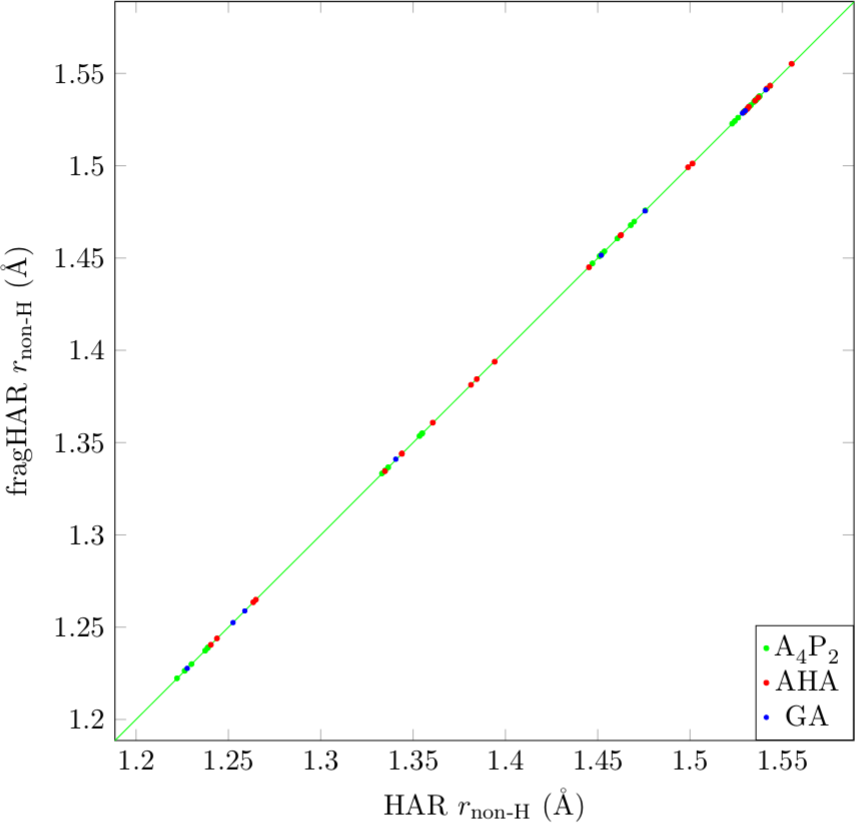
\includegraphics[width=0.8\linewidth]{graph_bond_non_H.png}
 \caption{Bond lengths between non-hydrogen atoms fragHAR 
 calculations plotted against reference HAR values. Error bars 
 are depicted, but are invisible to the eye on this scale.}
		\label{fig_bond_len_non_H}
\end{figure}
		

\begin{figure}
\centering
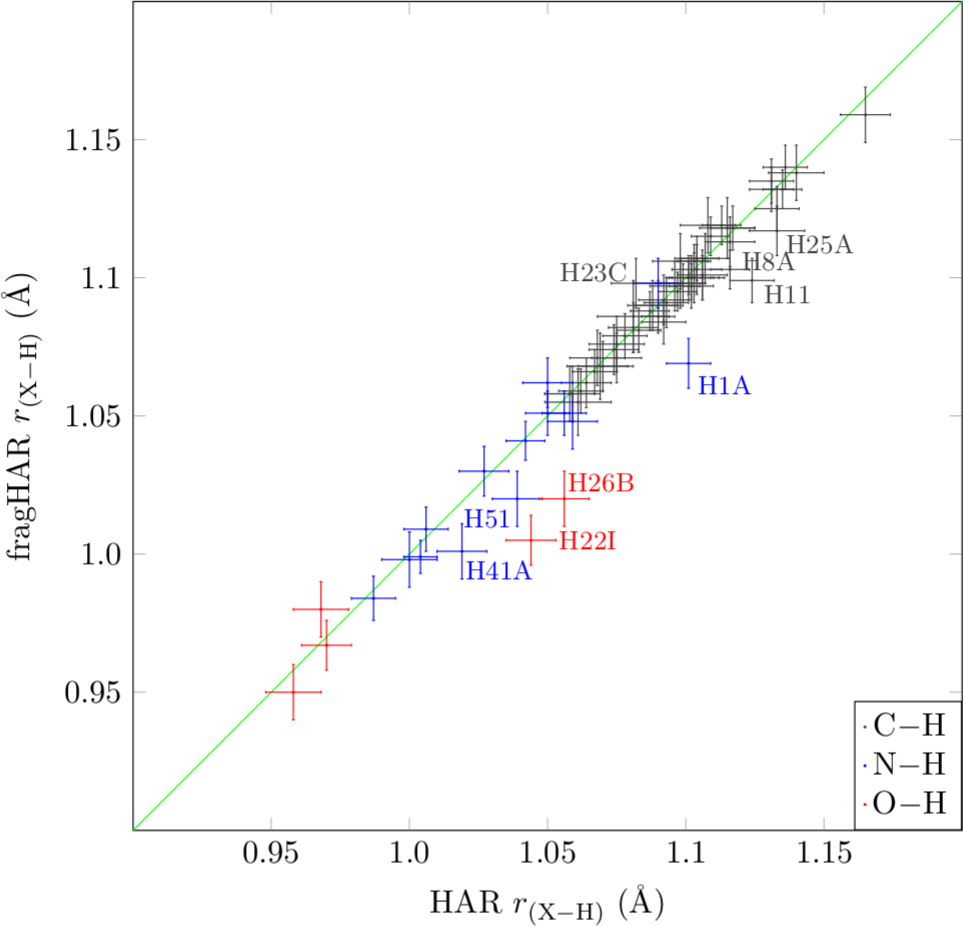
\includegraphics[width=0.6\linewidth]{graph_bond_H.png}
 
\caption{\ce{X-H} bonds (with error bars) in all model compounds,
        for fragHAR calculations versus reference HAR values. 
        Bonds with notable differences are marked with the 
        corresponding H atom name.}
		\label{fig_bond_len_H_bond_type}
\end{figure}


\begin{figure}
 \centering
 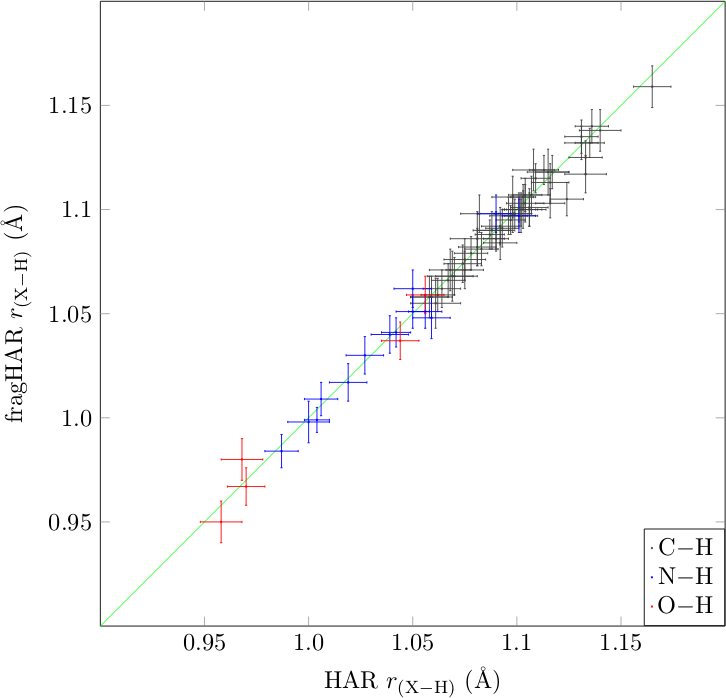
\includegraphics[width=0.6\linewidth]{bond_H_cor.png}
		\caption{\ce{X-H} bonds (with error bars) in all model compounds,
		for fragHAR with fragments ``joined'' across hydrogen bonds,
		versus reference HAR calculations.}
		\label{fig_bond_len_H_join_frag}
\end{figure}


%%%%%%%%%%%%%%%%%%%%%%%%%%%%%%%%%%%%%%%%
\subsection{Comparison of  atomic displacement parameters}

Table \ref{tbl_ADP} compares the ADPs obtained by fragHAR and HAR for non-hydrogen
and hydrogen atoms. For the non-hydrogen atoms, the mean absolute differences between
the ADPs from fragHAR and HAR are at least four orders of magnitude
smaller than the $w$RMSDs and the mean ratios are 0.999--1.000.
For the hydrogen atoms, the ratios  between the ADPs for the two types of refinement are 1.00--1.01 and the $w$RMSD is in range 0.2--0.6. Thus, the ADPs of the two methods are in statistical agreement.

\noindent
\begin{table}
\caption{Comparison of ADPs from fragHAR and HAR,
for non-hydrogen and hydrogen atoms. The diagonal and off-diagonal terms (three each) are treated separately. Values in brackets represent the sample 
standard deviations. \\}
\label{tbl_ADP}
\begin{tabular*}{\linewidth}{cllll}
\\
 \hline
&\multicolumn{4}{c}{Non-hydrogen atoms}\\
Compound
& $\langle U_{\s{fragHAR}}/U_{\s{HAR}} \rangle$ 
& $\langle |\Delta U_{ij}| \rangle$ 
& $\langle |\Delta U_{ii}| \rangle$ 
&$w$RMSD \\ 
\hline

GA	        &0.999(9) & 0.00006(7) & 0.00005(4) & 0.51 \\	
AHA         & 1.000(6) & 0.00005(6) & 0.00005(7) & 0.59 \\
 \ce{A4P2}  & 0.999(2) & 0.00001(2) & 0.00001(2) & 0.24 \\

& \\
 \hline
&\multicolumn{4}{c}{Hydrogen atoms} \\
&$\langle U_{\s{fragHAR}}/U_{\s{HAR}} \rangle$ 
&$\langle | \Delta U_{ij}| \rangle$ 
&$\langle | \Delta U_{ii}| \rangle$ 
&$w$RMSD \\ 
\hline

GA	            &	1.00(5) & 0.0007(6) & 0.0010(10) & 0.20 \\
AHA	            &	1.0(3) & 0.001(2) & 0.003(5) & 0.62 \\
 \ce{A4P2}       &  1.01(5) & 0.0005(6) & 0.000(2) & 0.19 \\
 \hline

  \end{tabular*}
  \end{table}

Although most ADPs from fragHAR and HAR refinements are in statistical agreement,
if they are plotted against each other, as in Figure \ref{fig_ADP_H}, 
a few ADPs with significant deviations can be observed.
 Again, these outliers are for hydrogen atoms involved in hydrogen bonds with other fragments.
The discrepancy also increase with the strength of the  
hydrogen bonds, so that there is a larger difference for the short hydrogen bonds than for the longer ones
(more details are given in the supplementary material). Again, it is 
interesting to see that the X-ray data contains enough information 
to distinguish these effects also in the ADPs, and even give some 
indication of their magnitude.
As seen for the bond lengths, the hydrogen ADPs are also improved if both fragments involved in hydrogen bonds are merged together in a single fragment (for example, $\langle | \Delta U_{ij}| \rangle$ for H41A decreases from 0.012  to 0.003.
%, compared to {\bf xxx} for HAR).
%{\justin{$U_{ij}$ H41A, HAR 0.029(4), fragHAR 0.037(5), join fragHAR 0.030(4)}}


\begin{figure}
 \centering
 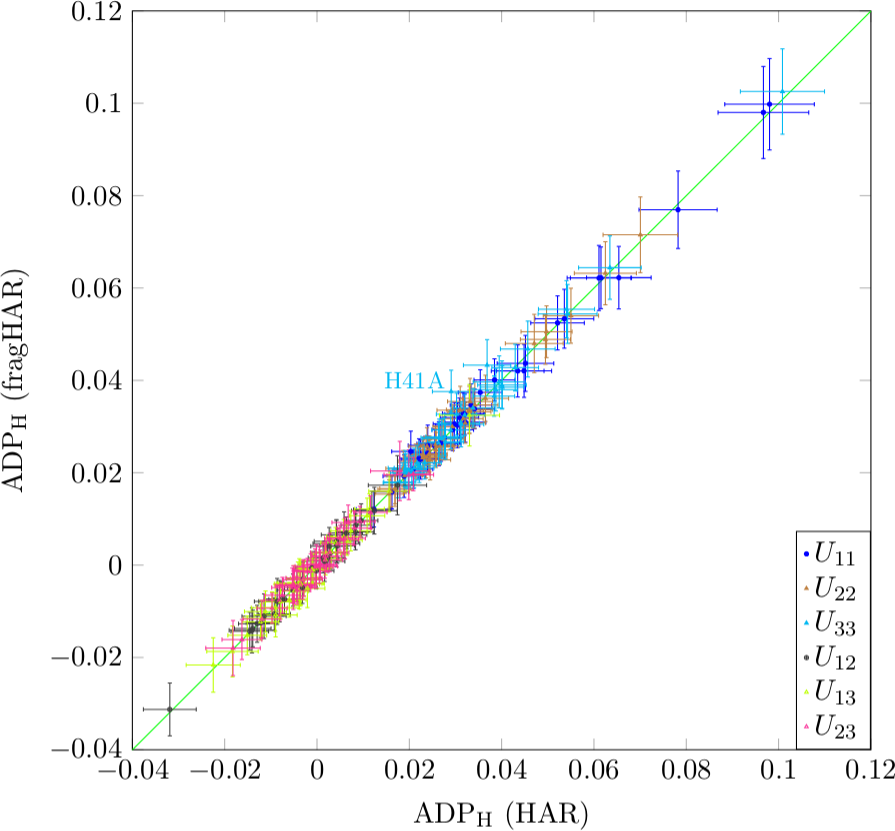
\includegraphics[width=0.8\linewidth]{graph_ADP.png}
	\caption{Hydrogen ADPs (with error bars) obtained with fragHAR 
	versus those from HAR for the \ce{A4P2} system. The hydrogen bonded
	H41A atom is labelled.}
	\label{fig_ADP_H}
\end{figure}







\subsection{Timing}
		
Figure \ref{fig_timing} shows the timings for HAR and fragHAR calculations
for single-processor (serial) and parallel calculations. fragHAR gives a significant 
reduction in calculation time for the bigger systems ({\em i.e.} those with more than
two fragments) for the serial calculations. 
When using parallel calculations, there is no difference
in time for the tripeptide because the time is \changed{determined} 
by the largest fragment
calculation. However, for the larger hexapeptide, fragHAR takes approximately 
half the time compared to HAR. Of course, even larger speed-ups are expected 
for larger systems \changed{since if every fragment is assigned its own processor 
in a large parallel system the wall time required for any size of protein will 
be constant}.

\begin{figure}
 \centering
 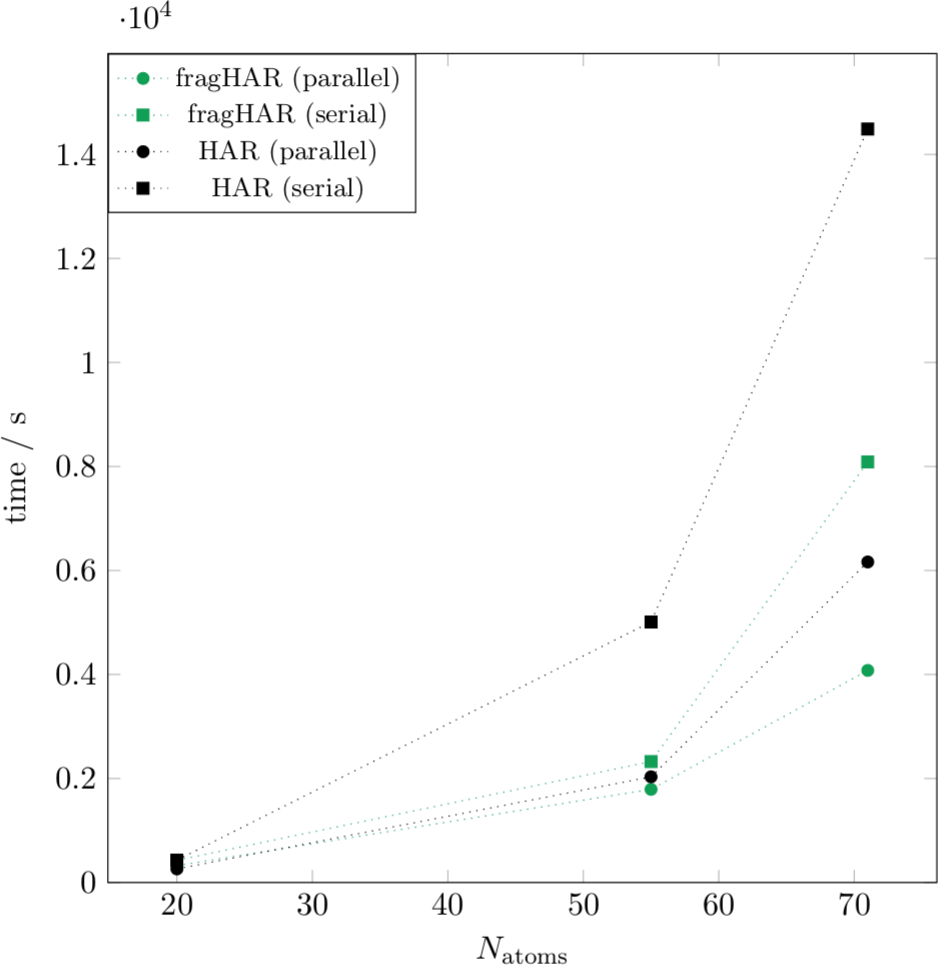
\includegraphics[width=0.8\linewidth]{graph_timing.png}
\caption{Timing of the fragHAR (in green) and HAR calculations (in black) 
for a single processor serial (square), and parallel calculations (circles)
for GA (2 processors),  AHA (4 processors) and \ce{A4P2} (4 processors). }
\label{fig_timing}
\end{figure}



\section{Conclusion}

We have described a method to improve the speed of Hirshfeld 
atom refinement (HAR) on peptides and proteins by breaking them 
up into capped residue fragments with the MFCC approach and performing wavefunction calculations
on those fragments. Based on tests on three oligopeptide systems, we show that the new
fragHAR method produces essentially the same $R$ factors, bond lengths and ADPs as  a full HAR calculation.
Significant differences are observed only for
hydrogen atoms involved in hydrogen bonds 
between the fragments. This problem can 
be fixed by enlarging the fragment to include the interacting group.


The fragHAR approach scales linearly with the size of the studied 
system and with a large-enough parallel computer, the calculations 
would take a fixed time, depending only on the length of the 
calculation on the largest fragment.

While ultra-high resolution data on proteins remains rare, there is a growing number 
of systems for which a resolution of  $<$0.8~\AA{}  can be obtained. 
Therefore the fragHAR method of quantum crystallographic 
refinement, which avoid the use of restraints, could contribute to determine 
hydrogen positions in proteins. 

Other serious problems remain to be solved. For example,
it remains to be shown what \changed{resolution will be needed
for the fragHAR method to give reliable H atom positions in proteins, 
because the effects of disorder may swamp any H atom signal.
The treatment of disorder is also somewhat tricky. Here,
the use of appropriate restraints and constraints to keep a 
chemically reasonable model will be important---some parts of 
a protein will always be disordered no matter quality of the data.
Still, it should be noted that fragHAR provides a natural solution 
to groups with alternative configurations, since one could use
a separate fragment for each conformation; by contrast, standard 
HAR would require separate calculations of the entire macromolecule 
for each alternative conformation}.

\changed{However, methods to treat disordered solvent by 
flattening  are well developed, as are methods to deal with 
constraints and restraints~\cite{sheldrick2015crystal}.
Also, we will shortly report an extension to HAR which 
treats disorder. With theses comments and the results of this 
paper in hand, there would seem to be good prospects to use 
fragHAR for  proteins where ultra-high resolution data can 
be obtained.}




\section{Acknowledgments}

This investigation has been supported by grants from the Swedish research council (project 2018-05003), from eSSENCE: the e-science collaboration and by an Australian Government Research Training Program Scholarship. 
The computations were performed on computer resources provided by the Swedish National Infrastructure for Computing (SNIC) at Lunarc at Lund University.




\bibliographystyle{iucr}
\bibliography{iucr}


\end{document}
